%
\documentclass[12pt]{article}

\usepackage{fullpage}
\usepackage{setspace}
\usepackage{endnotes}
%\usepackage{epsfig}
%\usepackage{psfrag}
\usepackage{amsmath}
\usepackage{amsfonts}
\usepackage{amssymb}
\usepackage{rotating}
\usepackage{dcolumn}
\usepackage{longtable}
\usepackage{microtype}
\usepackage{graphicx}
\usepackage{hyperref}
\usepackage[usenames,dvipsnames]{color}
%\usepackage{hypdvips}
\hypersetup{
 pdftitle={Compression and Conditional Effects}, % title
 pdfauthor={Redacted}, %Carlisle Rainey}, % author
 pdfkeywords={hypothesis testing}{interaction term}{product term}{interaction}{logit} {probit} {logisitic regression}
 pdfnewwindow=true, % links in new window
 colorlinks=true, % false: boxed links; true: colored links
 linkcolor=BrickRed, % color of internal links
 citecolor=BrickRed, % color of links to bibliography
 filecolor=BrickRed, % color of file links
 urlcolor=BrickRed % color of external links
}
\usepackage{url}
\usepackage{natbib}
%\bibpunct{(}{)}{,}{a}{}{;}
\usepackage{framed}
\usepackage{lipsum}
\usepackage[font=small,labelfont=sc]{caption}
 \usepackage{float}
\restylefloat{table}
\bibpunct{(}{)}{;}{a}{}{,}
\newtheorem{lemma}{Lemma}
\newtheorem{proposition}{Proposition}
\newtheorem{theorem}{Theorem}
\newtheorem{claim}{Claim}
\newenvironment{proof}[1][Proof]{\begin{trivlist}
\item[\hskip \labelsep {\bfseries #1}]}{\end{trivlist}}
\newenvironment{definition}[1][Definition]{\begin{trivlist}
\item[\hskip \labelsep {\bfseries #1}]}{\end{trivlist}}
\newenvironment{example}[1][Example]{\begin{trivlist}
\item[\hskip \labelsep {\bfseries #1}]}{\end{trivlist}}
\newenvironment{remark}[1][Remark]{\begin{trivlist}
\item[\hskip \labelsep {\bfseries #1}]}{\end{trivlist}}
%\newcommand{\qed}{\nobreak \ifvmode \relax \else
%      \ifdim\lastskip<1.5em \hskip-\lastskip
%      \hskip1.5em plus0em minus0.5em \fi \nobreak
%      \vrule height0.75em width0.5em depth0.25em\fi}
%      \setlength{\LTcapwidth}{5in}
%\def\p3s{\phantom{xxx}}

\usepackage{tgpagella}
\usepackage[T1]{fontenc}
%\usepackage[T1]{fontenc}
\usepackage[bitstream-charter]{mathdesign}


%Redefine the first level
\renewcommand{\theenumi}{\arabic{enumi}.}
\renewcommand{\labelenumi}{\theenumi}
%Redefine the second level
\renewcommand{\theenumii}{\alph{enumii}.}
\renewcommand{\labelenumii}{\theenumii}
%Redefine the third level
\renewcommand{\theenumiii}{\roman{enumiii}.}
\renewcommand{\labelenumiii}{\theenumiii}
%Redefine the fourth level
\renewcommand{\theenumiv}{\Alph{enumiv}.}
\renewcommand{\labelenumiv}{\theenumiv}


\parskip=0pt
\parindent=20pt
\usepackage{lscape}
\singlespace
\title{Compression and Conditional Effects}
%\author{Carlisle Rainey\thanks{Assistant Professor in the Department of Political Science at the University at Buffalo (SUNY)}}
\date{\today}
\usepackage[normalem]{ulem}

% Create footnote command so that my name
% has an asterisk rather than a one.
\long\def\symbolfootnote[#1]#2{\begingroup%
\def\thefootnote{\fnsymbol{footnote}}\footnote[#1]{#2}\endgroup}

\begin{document}


\begin{center}
\LARGE{\textbf{Compression and Conditional Effects\symbolfootnote[1]{Thanks to Kenneth Benoit, Bill Berry, Scott Clifford, Justin Esarey, and two anonymous reviewers for helpful comments on earlier versions of this manuscript. Thanks to John Oneal and Bruce Russet for making their data available. Thanks to the Center for Computational Research at the University at Buffalo for providing support for the simulations. Code and data necessary to replicate the simulations and empirical analysis is available at \href{http://www.carlislerainey.com/research}{http://www.carlislerainey.com/research} and at \href{http://thedata.harvard.edu/dvn/dv/PSRM}{http://thedata.harvard.edu/dvn/dv/PSRM}.}}}\\\vspace{4mm}

\normalsize{\textbf{A Product Term Is Essential When Using Logistic Regression to Test for Interaction}}\\\vspace{4mm}

\normalsize{\textsc{Carlisle Rainey\symbolfootnote[2]{Carlisle Rainey is Assistant Professor of Political Science, University at Buffalo, SUNY, 520 Park Hall, Buffalo, NY 14260 (\href{mailto:rcrainey@buffalo.edu}{rcrainey@buffalo.edu}).}}}\\\vspace{2mm}
\end{center}

\thispagestyle{empty}
%\end{document}
%\newpage
{\centerline{\textbf{Abstract}}}
\begin{quote}\noindent Previous research in political methodology argues that researchers do not need to include a product term in a logistic regression model to test for interaction if they suspect interaction due to compression alone. I disagree with this claim and offer analytical arguments and simulation evidence that when researchers incorrectly theorize interaction due to compression, models without a product term bias the researcher, sometimes heavily, toward finding interaction. However, simulation studies also show that models with a product term fit a broad range of non-interactive relationships surprisingly well, enabling analysts to remove most of the bias toward finding interaction by simply including a product term.\end{quote}
\thispagestyle{empty}
%\newpage
\singlespace
\setcounter{page}{1}

\doublespace

% Introduce the problem

\section*{Introduction}

Many theories in political science suggest an ``interactive'' relationship in which the effect of one explanatory variable $X$ depends on the value of another explanatory variable $Z$ \citep{ClarkGilliganGolder2006, BerryGolderMilton2012}. While earlier research lays out a clear and uncontroversial method for testing these claims in the context of \textit{linear} regression (e.g., \citealt{KamFranzese2007}; \citealt{BramborClarkGolder2006}; and \citealt{Friedrich1982}), political methodologists disagree about the best approach for researchers using \textit{logistic} regression, particularly over whether a product term must be included in the model (\citealt{Nagler1991}; \citealt{Frant1991}; \citealt{BerryBerry1991}; and \citealt{BerryDeMerittEsarey2010}).\footnote{Throughout the manuscript, I focus on logistic regression models in particular, but the conclusions generalize to a wide range of models of binary outcomes that rely on \textit{S}-shaped link functions, including probit models.}  

% Provide an overview of previous research 

The recent debate hinges around the substantive work of \cite{WolfingerRosenstone1980}, who theorize that easing registration restrictions should have a smaller positive effect on the probability of voting among individuals with more education. They do not evaluate the presence of interaction by testing the statistical significance of the product term's coefficient. Indeed, they do not even include a product term in the model. Instead, they simply note that, even without a product term, a logistic regression model can represent the kind of interaction suggested by their theory because the \textit{S}-shaped response curve creates ``compression,'' requiring that all variables have smaller effects as the probability of an event approaches zero or one. 

\begin{quote}\singlespace
As a statistical model, [logistic regression] is a more faithful representation of our substantive theory than [linear regression]. As we will see, the impact of most demographic variables is not constant across all types of individuals. Rather, the effect of a variable depends on the probability that the individual would vote. For example, a high-status occupation or a high income has less impact on a college graduate who is 90 percent likely to vote, than it has on a high school dropout, who is only 55 percent likely to vote... With [logistic regression] a variable has very little impact on those who are either very unlikely or nearly certain to vote. It has the greatest impact in the middle of the distribution, on those who are between 40 and 60 percent likely to vote and are the most susceptible to the forces pushing them to vote or not to vote (11).
\end{quote}

\noindent Instead of including a product term and testing the statistical significance of its coefficient, \cite{WolfingerRosenstone1980} argue for interaction by calculating a second-difference, which is the difference in the effect of easing registration restrictions between individuals with a high and low level of education. Formally, a second-difference $\Delta\Delta$ is the difference in the effect on $\text{Pr}(Y)$ of changing $X$ from a low value to a high value as $Z$ changes from a low value to a high value, which can be defined mathematically as follows:
\begin{align}
\Delta\Delta &= [\text{Pr}(Y | X = x_{hi}, Z = z_{hi}) - \text{Pr}(Y | X = x_{lo}, Z = z_{hi})]\nonumber \\
&-[\text{Pr}(Y  | X = x_{hi}, Z = z_{lo}) - \text{Pr}(Y  | X = x_{lo}, Z = z_{lo})], \nonumber
\end{align}
where $x_{lo}$, $x_{hi}$, $z_{lo}$, and $z_{hi}$ take on substantively interesting values of the explanatory variables $X$ and $Z$.\footnote{For more details, see \cite{BerryDeMerittEsarey2010}. For a discussion of using simulation to calculate confidence intervals for second-differences, see \cite{KingTomzWhittenburg2000} and \cite{HanmerKalkan2013} for an alternative.}  Using this approach, they find, as expected, that easing registration restrictions has a larger effect on the probability of turning out among less educated individuals. 

However, \citet[see \citeyear{Nagler1994} as well)]{Nagler1991} rejects this finding because the \textit{S}-shaped curve automatically builds interaction into the model. He claims that ``examining predicted probabilities generated by non-linear models such as [logistic regression] may produce spurious results when used to determine interactive effects between two [explanatory] variables (1393).'' Instead of just calculating a second-difference to quantify the amount of interaction, Nagler prefers to argue for interaction by including a product term and testing the statistical significance of its coefficient.  When he does this, the coefficient for the product of education and registration restrictions is incorrectly signed (suggesting that easing restrictions has a larger effect on the propensity to vote among the \textit{most} educated), leading Nagler to conclude that the data do not support Wolfinger and Rosenstone's theory. 

But \cite{BerryDeMerittEsarey2010} defend Wolfinger and Rosenstone's approach against Nagler's challenge, arguing that ``compression should not be viewed as theoretically irrelevant.'' Instead, they suggest that ``it can be a strong theoretical rationale for expecting interaction between variables in their influence on [the probability of an event] (255).'' Further, BDE suggest that if researchers expect interaction due to compression alone, then ``there is no need to include a product term in the model (261).'' In this situation, BDE recommend following Wolfinger and Rosenstone's strategy of (1) excluding a product term, (2) computing a second-difference, and (3) calculating a confidence interval and verifying that it contains only values consistent with the research hypothesis (i.e., is statistically significant).\footnote{Most of the debate about testing for interaction between two variables in influencing the probability of an event has occurred in political science. An earlier, but less detailed, debate between \cite{BerryBerry1990, BerryBerry1991} and \cite{Frant1991} almost exactly parallels the debate among \cite{WolfingerRosenstone1980}, \cite{Nagler1991}, and \cite{BerryDeMerittEsarey2010}. The substantive application focuses on lottery adoption in the U.S. states, but \cite{Frant1991} makes an argument similar to \cite{Nagler1991} and \cite{BerryBerry1991} make an argument similar to \cite{BerryDeMerittEsarey2010}. Also in political science, \cite{TsaiGill2013} and \cite{HuangShields2000} consider interaction in the context of logistic regression, but focus on the calculation of marginal effects on the probability of an event without addressing the need for a product term or discussing contexts in which researchers should care about the probability of an event as opposed to the latent outcome. While the most detailed discussions of interaction in the context of logistic regression have occurred in political science, especially relating quantities of interest and the need for a product term to substantive theories, similar discussions have emerged in related disciplines. Work in economics focuses on the relationship between the sign and significance of the product term in logit and probit models and the sign and significance of the second-derivative  $\dfrac{\partial^2 \text{Pr}(Y)}{\partial X \partial Z}$ (\citealt{AiNorton2003}; \citealt{NortonWangAi2004}; and \citealt{Greene2010}). However, this work offers little guidance as to when applied researchers should focus on $\dfrac{\partial^2 \text{Pr}(Y)}{\partial X \partial Z}$ as opposed to $\dfrac{\partial^2 Y^*}{\partial X \partial Z}$ and does not discuss the consequences of including or excluding a product term. Research in epidemiology works to define interaction in the context of logistic regression models, usually focusing on differences in risk-ratios rather than second-differences or second-derivatives. Again, though, this literature offers little guidance about whether researchers should include or exclude a product term in logistic regression models used to test for interaction. Also outside of political science, \cite{Bowen2012} draws a sharp distinction between the interaction induced by the inclusion of a product term and the interaction induced by the link function and offers a statistical test to distinguish the two forms of interaction, but does not address whether a product term is necessary to conclude that interaction is present and does not offer advice about the advantages of focusing on the probability of an event instead of the latent outcome variable.}

Despite compression's theoretical relevance, I argue that researchers should \textit{always} include a product term, even when they expect interaction on the basis of compression alone. A product term is not necessary to allow the model to represent interaction--it can do that with no product term \citep{BerryDeMerittEsarey2010}. A product term must be included because it allows the model to better represent a \textit{non-interactive} relationship. I present an analytical argument and simulations showing that if no product term is included, a logistic regression model cannot represent a non-interactive relationship and thus overstates the evidence for interaction. Fortunately, I find that simply including a product term eliminates most of this bias.

\section*{Current Advice to Applied Researchers}

Prior to the publication of \cite{BerryDeMerittEsarey2010}, the literature suggested that when analysts faced a dichotomous outcome and suspected interaction, there was only one path forward: include a product term and conclude that there is interaction between $X$ and $Z$ if and only if the coefficient for the product term was statistically significant \citep[though see \citealt{BerryBerry1991}]{Nagler1991, BramborClarkGolder2006}. However, Berry, DeMeritt, and Esarey (\citeyear{BerryDeMerittEsarey2010}, \citeyear{BerryDeMerittEsarey2014}) have added much needed nuance to this advice. In particular, \cite{BerryDeMerittEsarey2010} lay out an initial framework describing the contexts in which researchers should hypothesize in terms of the latent variable $Y^*$ or $\text{Pr}(Y)$, describe the implications for whether one performs hypothesis tests on the coefficient of the product term or a second-difference, and make suggestions about when to include a product term. Table \ref{tab:lit} synthesizes the advice from \cite{Nagler1991}, \cite{BerryDeMerittEsarey2010}, and \cite{BerryDeMerittEsarey2014}, summarizing the current advice to applied researchers.

\renewcommand{\arraystretch}{1.5}
\begin{table}
\begin{center}
\begin{scriptsize}
\begin{tabular}{|>{\centering\arraybackslash}m{1in}m{2in}>{\centering\arraybackslash}m{.7in}>{\centering\arraybackslash}m{.5in}>{\centering\arraybackslash}
m{1.2in}|}
\hline

Situtation &
\begin{center}
Description
\end{center} & Include a Product Term? & Quantity of Interest & Source\\ 
\hline
Interaction in Influencing the Latent Outcome & Guided by a strong theory, the analyst hypothesizes that $X$ and $Z$ interact in influencing the latent outcome variable $Y^*$. For example, it sometimes makes sense to conceptualize $Y^*$ as utility and derive a probit model using a random utility framework \citep{Train2009}. See \citet[esp.pp. 261-262]{BerryDeMerittEsarey2010} for more details and an example. & Yes & $\dfrac{\partial^2 Y^*}{\partial X \partial Z}$ & \cite{Nagler1991}\\ 
Interaction Due to Compression Alone & Guided by a strong theory, the analyst hypothesizes that $X$ and $Z$ interact in influencing $\text{Pr}(Y)$ due to compression alone. That is, as the probability of an event approaches zero or one, the effect of any explanatory variable (including $X$ and $Z$) have smaller effects. While researchers such as \cite{Frant1991} and \cite{Nagler1991} sometimes dismiss compression as an unimportant form of interaction, \cite{BerryDeMerittEsarey2010} make a strong case that this type of interaction is often theoretically meaningful. & \underline{\textbf{No}} & $\dfrac{\partial^2 \text{Pr}(Y)}{\partial X \partial Z}$ & \cite{BerryDeMerittEsarey2010}\\ 
Specification Ambiguity & Guided only by weak theoretical intuition, the analyst hypothesizes that $X$ and $Z$ interact in influencing $\text{Pr}(Y)$, but have no strong theoretical rational for the functional form. In this situation, the analyst lacks the theoretical guidance necessary to theorize about interaction in terms of the latent variable or on the basis of compression alone.  & Yes & $\dfrac{\partial^2 \text{Pr}(Y)}{\partial X \partial Z}$& \cite{BerryDeMerittEsarey2014} \\ 
\hline
\end{tabular}\caption{This table summarizes three situations in which analysts might theorize interaction in the context of logistic regression. Notice that the quantity of interest varies across these situations, as well as whether the literature recommends including a product term. In this paper, I address the situation in which an analyst suspects interaction due to compression alone. In particular, I agree with Berry, DeMeritt, and Esarey's (2010) characterization of the theoretical value of compression and the implied quantity of interest, but argue that analysts must still include a product term.}\label{tab:lit}
\end{scriptsize}
\end{center}
\end{table}

I find the advice in Table \ref{tab:lit} sound, useful, and large improvement over the coarse practice prior to \cite{BerryDeMerittEsarey2010}. However, I disagree with the recommendation to exclude a product term when the analyst puts forward a strong theory predicting interaction on the basis of compression alone (the bold ``No'' in Table \ref{tab:lit}). In this paper, I explain why I find Berry, DeMeritt, and Esarey's (\citeyear{BerryDeMerittEsarey2010}) argument for excluding a product term incomplete.

\section*{The Argument for Excluding a Product Term}

Berry, DeMeritt, and Esarey's (\citeyear{BerryDeMerittEsarey2010}) (hereafter, BDE) overarching claim, which I wholeheartedly agree with, is that ``a statistically significant product term is neither necessary nor sufficient for concluding that there is substantively meaningful interaction among independent variables in their influence on [the probability of an event]'' (261). Given this point though, BDE ask whether it is always necessary to include a product term in the model. To decide whether to include a product term, they suggest that analysts draw a sharp distinction between theories that focus on the unbounded latent variable, denoted as $Y^*$ (perhaps conceptualized as ``utility''), and theories that focus on the probability of an event, denoted as $\text{Pr}(Y)$.\footnote{In BDE's notation, $Y^*$ refers to the so-called ``latent variable'' implied in models of binary outcomes. $Y^*$ simply equals the value of the linear predictor, often denoted by $\eta = X\beta = \beta_0 + \beta_1X_1 + \beta_2X_2 + ... + \beta_kX_k$ in the notation of generalized linear models, and is transformed into $\text{Pr}(Y)$ by an inverse link function that maps the real line to $[0, 1]$. Sometimes researchers' theories lead to hypotheses about $Y^*$ rather than $\text{Pr}(Y)$. For example, theorists often link formal models of decision-making to random utility models, a common framework for deriving models such as logistic regression, particularly the almost identical probit model. Using this approach, researchers can evaluate explanations of utility, represented by the value of $Y^* = \eta = X\beta$.}

\begin{quote}\singlespace
\textit{BDE Recommendation}: When guided by a strong theory, the decision to include a product term must be based on the theorized effects of variables on the unbounded latent dependent variable $Y^*$, assumed by the model.\vspace{2mm}\\
\indent \textit{Part (a)}: If the theory assumes that variables interact in influencing the latent unbounded variable $Y^*$, then the researcher should include a product term. (See the situation ``Interaction in Influencing the Latent Outcome'' in Table \ref{tab:lit}.)
\end{quote}
\doublespace
We agree on \textit{Part (a)}. As both BDE and \cite{Nagler1991} note, this situation is entirely analogous to linear regression (e.g.,  $Y^* = \beta_0 + \beta_1X_1 + \beta_2X_2 + ... + \beta_kX_k )$, making a product term essential.
\begin{quote}\singlespace
\indent \textit{Part (b)}: If the theory assumes that variables should interact in influencing $\text{Pr}(Y)$ strictly on an expectation of compression, then there is no need to include a product term in the model. (See the situation ``Interaction Due to Compression Alone'' in Table \ref{tab:lit}.)
\end{quote}\doublespace
BDE explain:
\begin{quote}\singlespace 
[I]n any logit or probit model, the marginal effect
of $X$ on $\text{Pr}(Y)$ depends on the values of all [explanatory]
variables; this marginal effect is greatest when $\text{Pr}(Y)$ is
0.5 and declines when a change in either variable pushes
$\text{Pr}(Y)$ toward 0 or 1. We refer to the phenomenon ... as compression,
because deviations of $\text{Pr}(Y)$ away from [0.5] compress
further possible change in \text{Pr}(Y) to ever-smaller ranges.
 (251)
 \end{quote}\doublespace
They continue by suggesting:
\begin{quote}\singlespace
[A] researcher...may base his hypothesis that independent variables interact in influencing $\text{Pr}(Y)$ strictly on an expectation of compression. In this case, there is no need to include a product term in the model. Put differently, no product term is required if the analyst's only reason for positing interaction between $X$ and $Z$ in influencing $\text{Pr}(Y)$ is an expectation that when the value of $X$ is extreme, $\text{Pr}(Y)$ is near its limit of zero or one and thus there is little room for $\text{Pr}(Y)$ to change as $Z$ changes. In any event, the analyst should use the parameter estimates for the model (with no product term) to generate estimates of the effects of variables on $\text{Pr}(Y)$ to test his hypothesis; the same tools used for models with a product term--second-differences or marginal effect plots--can be employed.
(261)
\end{quote}
\doublespace
While I find BDE's suggestion to exclude a product term problematic, I take two other points from their paper as a starting point.
\begin{enumerate}
\item Compression can be substantively interesting and theoretically meaningful. Consider the example from \cite{WolfingerRosenstone1980} discussed above. Recall that their model does not have a product term, the only interaction is due to compression. Yet if their model is correct , then restrictive voting rules not only reduce turnout, but also increase the inequality of political participation because restrictive rules have a larger negative effect on the probability of voting among the least educated. This relationship has  enormous normative consequence and policy relevance.
\item If analysts are interested in interaction due to compression, then the quantity of interest is not the product term, but the second-difference (or second-derivative). Several authors show that the sign and significance of the second-difference does not depend on the sign and significance of the product term (e.g., \citealt{TsaiGill2013, AiNorton2003}).
\end{enumerate}
 Although, I find BDE's argument for these two points compelling, I disagree with the advice to exclude a product term when theorizing interaction on the basis of compression alone.

\section*{The Argument for Including a Product Term}

Researchers must employ a statistical model that can represent (1) relationships that are \emph{consistent} with the theory and (2) plausible relationships that are \emph{inconsistent} with the theory. It is obvious that models should be able to represent relationships that are consistent with theory. But if researchers use models that cannot also represent situations \emph{inconsistent} with the theory, then they have assumed their theories are correct. Though the theoretical rationale may be strong, it has not been made vulnerable to the data.

Thus, BDE's analysis is incomplete when they write that ``no product term is required if the analyst's only reason for positing interaction between $X$ and $Y$ in influencing $\text{Pr}(Y)$ is an expectation that when the value of $X$ is extreme, $\text{Pr}(Y)$ is near its limit of zero or one, and thus there is little room for $\text{Pr}(Y)$ to change as $Z$ changes.'' While they correctly note that the theorized relationship can be represented by a model with no product term, they fail to discuss whether this model can also represent relationships that are inconsistent with the theory.

Without a product term, a logistic regression model cannot represent many reasonable situations that are inconsistent with an interactive theory. In particular, it cannot represent a situation in which two explanatory variables have non-zero effects and the probability of an event is greater or less than one-half, but there is no interaction. Specifically, for a logistic regression model including $X$ and $Z$, but excluding their product, if all of the following conditions hold, then $X$ and $Z$ must interact in influencing Pr$(Y)$. \footnote{For further discussion, see \cite{Nagler1991} and \cite{BerryDeMerittEsarey2010}.}
\begin{enumerate}
\item $X$ has a non-zero effect.
\item $Z$ has a non-zero effect.
\item $\text{Pr}(Y) < 0.5$ or $\text{Pr}(Y) > 0.5$.
\end{enumerate}

This can easily be seen by inspecting the second derivative of the logistical regression model with no product term, given by 
\begin{align}
\dfrac{\partial^2 \text{Pr}(Y)}{\partial X \partial Z} &=  \text{Pr}(Y)[1 - \text{Pr}(Y)][1 - 2\text{Pr}(Y)]\beta_x \beta_z. \label{eqn:dnoprod}
\end{align}
If any of Conditions 1-3 hold, then the second derivative is exactly zero. Otherwise, the second derivative is non-zero, which implies an interactive relationship the model. Consequentially, if the researcher incorrectly theorizes compression, but 1-3 hold, then a logistic regression model without a product term will overstate the evidence for interaction.\footnote{Responding to Frant's (\citeyear{Frant1991}) suggestion to include a product term, \cite{BerryBerry1991} write: 
\begin{quote}
Frant claims that this result [that the effect of election proximity on the probability of lottery adoption depends on the state's fiscal health] ``sounds like a \textit{conclusion} (and the authors' treat it as such); but it is actually an \textit{assumption} of the model.'' It is true that interaction among among variables in their effects on the probability of adoption is an assumption of our probit model. But all multivariate models make assumptions about the function form of effects of independent variables; yet substantive conclusions are drawn from empirical analyses of these models. Indeed, an interactive regression with a multiplicative term (e.g., $E(Y) = \beta_0 + \beta_1X_1 +\beta_2X_2 + \beta_3X_1X_2$)--similar to the form that Frant proposes we use--also \textit{assumes} interaction among the independent variables (provided $\beta_3 \neq 0$) (574). 
\end{quote}
My analytical argument supports Frant's (\citeyear{Frant1991}) position. While \cite{BerryBerry1991} are correct that the linear model including a product term assumes a form of interaction (e.g., the marginal effect of $X_1$ is a \textit{linear} function of $X_2$), it does not assume that interaction is present (hence their caveat that $\beta_3 \neq 0$). A linear model with a product term can represent situations that are consistent and inconsistent with the interactive theory ($\beta_3 \neq 0$ and $\beta_3 = 0$, respectively). This allows the model to effectively assess the evidence against the null hypothesis and for the research hypothesis. As the analytical argument shows, the logistic regression model with no product term, while it can represent an interactive relationship, cannot represent a non-interactive relationship. Both my anlytical arguments and simulations strongly suggest that \cite{Frant1991} is correct when he advises researchers to avoid making empirical claims about interaction between variables in influencing the probability of an event when no product term is included in the model.} 

With a product term, however, a logistic regression model can represent \textit{some} plausible situations inconsistent with an interactive theory. For a logistic regression model including $X$, $Z$, and $XZ$, if all of the conditions (1-3) identified above hold, then $X$ and $Z$ \textit{may or may not} interact in influencing Pr$(Y)$. The intuition of this claim can be seen by simply inspecting the second derivative of a logistic regression model including a product term, given by
\begin{equation}
\begin{aligned}
\dfrac{\partial^2 \text{Pr}(Y)}{\partial X \partial Z} &= \text{Pr}(Y)[1 - \text{Pr}(Y)]\beta_{xz} \\
&+ \text{Pr}(Y)[1 - \text{Pr}(Y)][1 - 2\text{Pr}(Y)](\beta_x + \beta_{xz}Z )(\beta_z + \beta_{xz}X)\label{eqn:dprod}. 
\end{aligned}
\end{equation}
The presence of the product term creates another coefficient that allows the second derivative to be zero, even if Conditions 1-3 hold. Thus, this model is capable of representing situations in which 1-3 hold, but no interaction is present. This means that a product term ``uncouples'' hypotheses about  the effects of $X$ and $Z$ from their interaction.

While including a product term does not entirely remove the bias toward confirming interactive hypotheses, it does greatly reduce the bias. Thus, including a product term makes the empirical argument more compelling by making the theory more vulnerable to the data.\footnote{This analytical argument provides a formal justification for Huang and Shield's (\citeyear{HuangShields2000}) claim that ``[o]f course, adding multiplicative terms to explicitly model this interactive relationship is necessary (86).''}

\section*{Simulations}

To illustrate the potential consequences of excluding a product term, I report two simulation studies. The first examines a single relationship in detail. The second looks at a wide range of potential relationships. Because I am particularly interested in what happens if the theory (or researcher's hypothesis) is wrong, I imagine that a researcher incorrectly theorizes interaction due to compression and follows BDE's suggestion to exclude the product term. In almost all cases, excluding the product term biases the researcher toward finding support for her theory.

But why focus specifically on what happens if the researcher is wrong? Why not look at what happens if the researcher correct theorizes interaction on the basis of compression alone? Careful readers recognize the tradeoff between the size of a hypothesis test (i.e., the probability of finding interaction when there is none) and power (i.e., the probability of finding interaction when it is present). While analysts usually face a tradeoff between these two, I focus my attention squarely on the size of tests for interaction.

Hypothesis test form compelling statistical arguments because, by design, they rarely lead a researcher to reject the null hypothesis when they null hypothesis is true. This is because hypothesis tests are constructed by fixing $\alpha = \text{Pr}(\text{reject null} | \text{null is true})$  at an acceptably low value, typically $\alpha = 0.05$. This is important because researchers and readers interpret decision to reject the null hypothesis as strong evidence against the null hypothesis (or for the research hypothesis).

Social scientists typically use hypothesis tests because they want to conclude that their research hypothesis is correct \underline{only} when the data offer strong evidence in favor of their research hypothesis (or equivalently, against their null hypothesis). If a test is improperly sized (e.g., $\alpha = 0.75$), then the decision to reject the null hypothesis is no longer compelling. Making matters worse, readers and reviewers are still likely to interpret the results of this over-sized test as compelling. I focus squarely on the size of tests for interaction because the logic of hypothesis testing requires that the size be fixed at a suitably small value, usually 0.05 in the social sciences, while allowing the power of a test to fluctuate with other variables, such as the number of observations. My primary focus on size, or Type-I or false-positive errors, should not be taken as meaning that power is unimportant. To address the secondary issue of power, I include a discussion of the statistical power of models that exclude and include product term in the Appendix. These simulations reported in the Appendix show that the ability of a model with a product term to ``detect'' an interactive relationship (i.e., statistical power) is nearly equal if the amount of interaction is substantial or the sample size is large. However, it is important to point out that when the sample size is small (e.g., less than 1,000) \textit{and} the amount of interaction is small (e.g., second-difference of $0.04 - 0.09 = -0.05$), then including a product term might lead to a substantial drop in statistical power. However, it is important to note that the gain in statistical power comes from \textit{assuming} an interactive relationship, not \textit{detecting} one.

One might also worry about the impact of including a potentially unnecessary product term $XZ$ in the model (i.e., $\beta_{XZ} = 0$) on the estimated effects of other variables in the model. In the Appendix, I show that including an unnecessary product term does not lead to bias in the estimated effects of other variables in the model.

\subsection*{Study \#1: A Fixed Relationship} 

I first consider the non-interactive relationship (i.e., data-generating process) $\text{Pr}(Y) = 0.3 + 0.2X - 0.3Z$ shown in the left panel of Figure \ref{fig:relationships-fits}. I imagine that the analyst correctly suspects that $X$ has a positive effect on $\text{Pr}(Y)$ and $Z$ has a negative effect on $\text{Pr}(Y)$.  She also theorizes that because the event is relatively rare and $Z$ pushes $\text{Pr}(Y)$ even closer to zero,  there is less room for $X$ to affect $\text{Pr}(Y)$. Therefore, she expects that $X$ should have a smaller effect when $Z=1$. But this hypothesis is not correct--she \textit{incorrectly} expects that $X$ and $Z$ interact in influencing $\text{Pr}(Y)$ due to compression. Still, she notices that a logistic regression model can represent the kind of interaction suggested by her theory and decides that no product term is necessary \citep{BerryDeMerittEsarey2010}. 

Because $X$ is approximately uniformly distributed from zero to one and $Z$ is dichotomous with half of the observations equal to one and the other half equal to zero, she decides to test for interaction by estimating a logistic regression model with no product term, calculating the second-difference as $X$ changes from 0.25 to 0.75 and $Z$ changes from zero to one. Her hypothesis suggests that this second-difference should be negative, since $X$ should have a smaller effect when $Z=1$.

\begin{figure}[H]
\begin{center}
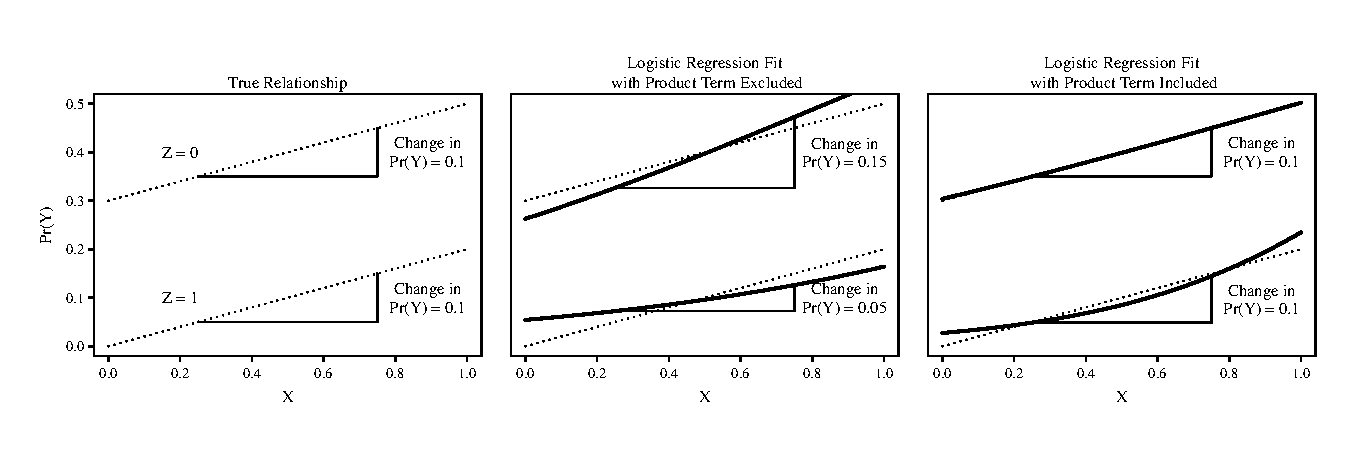
\includegraphics[width=\linewidth]{fig/fig-example.pdf}
%\vspace{-10mm}
\end{center}
\caption{This figure shows the true relationship in the first simulation study (dotted lines) as well as how logistic regression models with and without a product term fit the process (solid, bold lines). Notice that $X$ and $Z$ have large effects on $\text{Pr}(Y)$ and $\text{Pr}(Y)$ is always less than 0.5. In this case, excluding a product term forces the model to point toward interaction, despite the fact that the relationship is non-interactive. Including a product term allows the model to fit this non-interactive process surprisingly well.}\label{fig:relationships-fits}
\end{figure}

Notice the middle panel of Figure \ref{fig:relationships-fits}, which shows how a logistic regression model without a product term might fit the true relationship. Although there is no interaction in the actual data-generating process, the logistic regression model with no product term suggests that there is  substantial interaction between $X$ and $Z$ in influencing $\text{Pr}(Y)$. When $Z=1$, the estimated effect of moving $X$ from 0.25 to 0.75 is 0.05. When $Z=0$, however, the effect of $X$ triples to 0.15 (the second-difference is $0.05 - 0.15 = -0.1$). Although the hypothesis of interaction is wrong, the logistic regression model with no product term suggests there is strong evidence in favor of it.

Now notice the right panel of Figure \ref{fig:relationships-fits}, which shows the estimates when the model contains a product term. While this model does not exactly capture the true data-generating process (i.e., notice the non-linearity when $Z = 1$), it estimates the amount of interaction very well. The estimated effect of $X$ when $Z=0$  is 0.1. When $Z = 1$, the estimate is identical. Therefore, the estimated second-difference is zero ($0.1 - 0.1 = 0$) and the model correctly suggests that there is no interaction.

Rather than examining how models fit the data-generating process, it is perhaps more informative to evaluate each approach in repeated trials. To do this, I simulate 3,000 data sets containing 1,000 observations each. I use each data set to estimate a second-difference and its confidence interval using a model with and without a product term. Finally, I estimate $\alpha = \text{Pr}(\text{Find Interaction})$, the probability of finding interaction \textit{when none is present} (i.e., a Type-I or false-positive error), by calculating the proportion of data sets that pointed toward interaction with each approach (i.e., the confidence interval does not contain zero). By convention, this probability should be close to 0.05. When the model does not include a product term, the probability of finding interaction is 0.98. Thus,  finding a statistically significant second-difference is not a all  compelling evidence against the null when the model does not include a product term, since the researcher will likely find this even when there is no interaction. However, the probability of finding interaction drops to 0.06 when the researcher includes a product term in the model. This suggests that finding a statistically significant second-difference is compelling  when the model includes a product term since the researcher would rarely find this when the null is true.

To help understand why excluding a product term biases the researcher toward finding interaction, Figure \ref{fig:plotted-cis} shows the estimates and confidence intervals from only 50 simulated data sets, sorted by the size of the estimated second-difference. Notice the left panel of Figure \ref{fig:plotted-cis}, which shows that the models without a product term always estimate a substantial amount of interaction in the expected direction  and that the confidence intervals rarely overlap zero. \textit{This happens because compression serves as the theoretical motivation for the hypothesis and is \underline{assumed} by the model.} But notice the right panel of Figure \ref{fig:plotted-cis}, which shows that most of this bias disappears when a product term is included in the model.

\begin{figure}[h]
\begin{center}
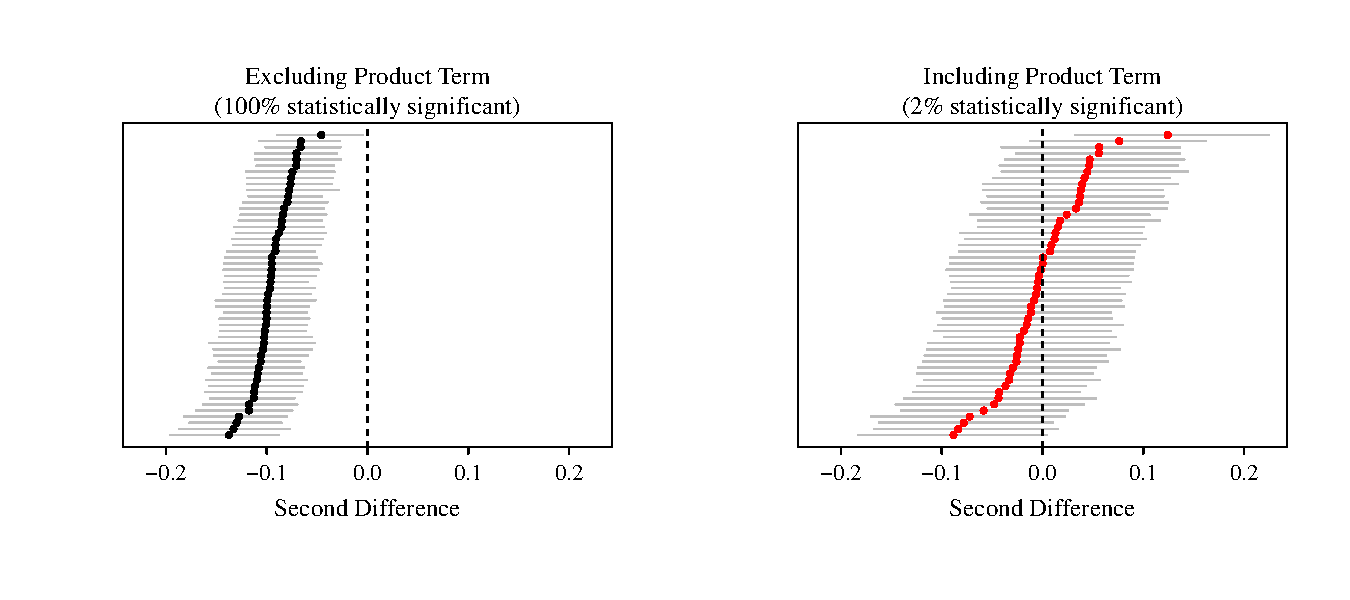
\includegraphics[scale=.7]{fig/fig-plotted-cis.pdf}
%\vspace{-10mm}
\end{center}
\caption{This figure shows fifty simulations of estimated second-differences and confidence intervals using models with and without a product term. Although second-difference is actually zero (a non-interactive relationship), the model with no product term consistently finds interaction. Including a product term removes almost all of this bias.}\label{fig:plotted-cis}
\end{figure}

To get a sense of the robustness of this conclusion, I systematically vary the sample size, the distribution of $X$, and the change in $X$ used to calculate the second-difference while the true relationship remains the same. For each combination of the simulation parameters, I simulate 3,000 data sets. For each data set, I estimate a logistic regression model with and without a product term and compute the confidence interval around the second-difference, as BDE recommend. I then calculate the proportion of simulations in which each model points incorrectly toward interaction to estimate the probability of finding interaction when none is present. The results are presented in Figure \ref{fig:fixed}.

Across all values of the simulation parameters, the models without a product term bias the researcher toward finding interaction and sometimes strongly. The bias is reduced, usually dramatically, when the researcher includes a product term. Indeed, for symmetric distributions of $X$ and centered second-differences, adding a product term to the model eliminates nearly all of the bias, lowering the probability of finding interaction
from nearly 1.00 (the worst  situation) to about 0.05 (the ideal situation).\footnote{As a robustness check, I repeated this study using a slight different data generating process. For this alternative, ``rare events'' process, the probability of an event never rises above 0.08. The full results are discussed in the Appendix, but the basic findings suggest an even more optimistic conclusion about the ability of the product term to remove the bias toward finding interaction. This is as expected since I chose the fixed process discussed above to serve as a worst case scenario.}

\begin{figure}
\begin{center}
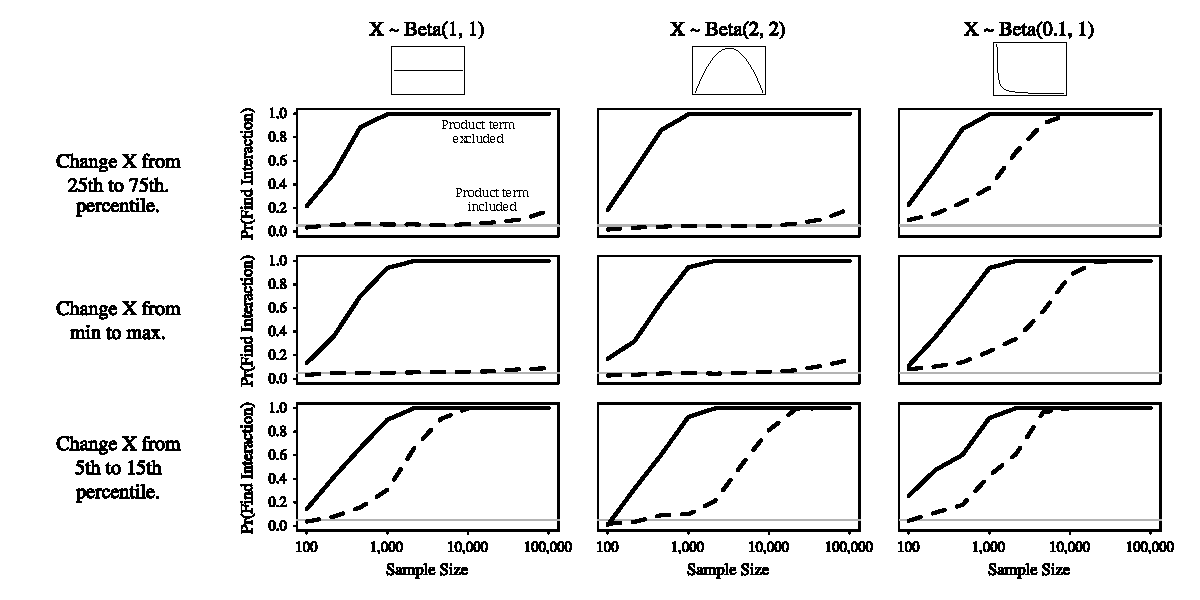
\includegraphics[width=\linewidth]{fig/fig-fixed.pdf}
\end{center}
\caption{This figure shows the probability of concluding interaction when the true relationship is given by $\text{Pr}(Y) = 0.3 + 0.2X - 0.3Z$ (i.e., there is no interaction) using logistic regression models with and without a product term as the sample size, the distribution of $X$, and the change in $X$ considered in computing the second-difference varies. Notice that the model including a product term performs remarkably well, although the improvement diminishes as the simple size gets large, especially when the distribution of $X$ is skewed and the researcher considers the effect of changing $X$ nears its extremes.}\label{fig:fixed}
\end{figure}

\subsection*{Study \#2: A Diverse Set of Relationships}

To demonstrate that the patterns seen in Figure \ref{fig:fixed} do not depend on any particular relationship, I now examine a diverse collection of 1,500 simulated analyses. Each analysis is generated through a random process (described in the Online Appendix) that varies in the following ways:\singlespace\vspace{-3mm}
\begin{enumerate}
\item The relationship between $\text{Pr}(Y)$, $X$, and $Z$ varies, but follows the form of $\text{Pr}(Y) = \beta_0 + \beta_1X + \beta_2Z + \beta_3X^2 + \beta_4Z^2$ and is always monotonic across the range of $X$ and $Z$. Importantly, $X$ and $Z$ never interact in changing $\text{Pr}(Y)$.\footnote{I use a quadratic functional form here to include a more general set of curves rather than restrict my processes to straight lines. The only condition that I want to place on the processes is that they be monotonic (i.e., the marginal effects never change signs) and there be no interaction. The quadratic form allows a nice mixture of different relationships within these restrictions (though not exhaustive, of course). The restriction disallowing interaction is necessary because I am interested mainly in the probability of finding interaction when their is none present.}
\item The distributions of $X$ and $Z$ vary and might be binary, flat, unimodal, or  skewed to the right.
\item The values of $x_{lo}$, $x_{hi}$, $z_{lo}$, and $z_{hi}$ used to construct the second-difference vary from zero to one. All combinations are possible, though if a variable is binary, its values are set to zero and one.
\item The sample size varies, ranging from 500 to 100,000, though smaller samples are more likely.


\end{enumerate}
\doublespace
Each ``analysis'' consists of features the researcher totally controls (e.g., values of $x_{lo}$, $x_{hi}$, $z_{lo}$, and $z_{hi}$), somewhat controls (e.g., sample size), and does not control (e.g., distributions of explanatory variables and the true data-generating process). For each simulated analysis, I use the same procedure as before to estimate the probability of finding interaction using models with and without a product term. Because none of the true relationships are interactive, this probability should be near 0.05. 

The left panel of Figure \ref{fig:hist} shows that when the researcher uses a logistic regression model without a product term, the probability of finding interaction when none exists is less than 0.1  for  only 40 percent of the simulated analyses. It is greater than 0.9 for over 20 percent of the analyses. This suggests that excluding a product term strongly biases the researcher toward finding interaction for many plausible relationships. On the other hand, the right panel of Figure  \ref{fig:hist} shows that, when using a model with a product term, the probability of finding interaction is less than 0.1  for almost all of the simulated analyses  (over 98 percent).
This suggests that including a product term can eliminate most of the bias toward finding interaction for many plausible relationships and analyses.

\begin{figure}[h]
\begin{center}
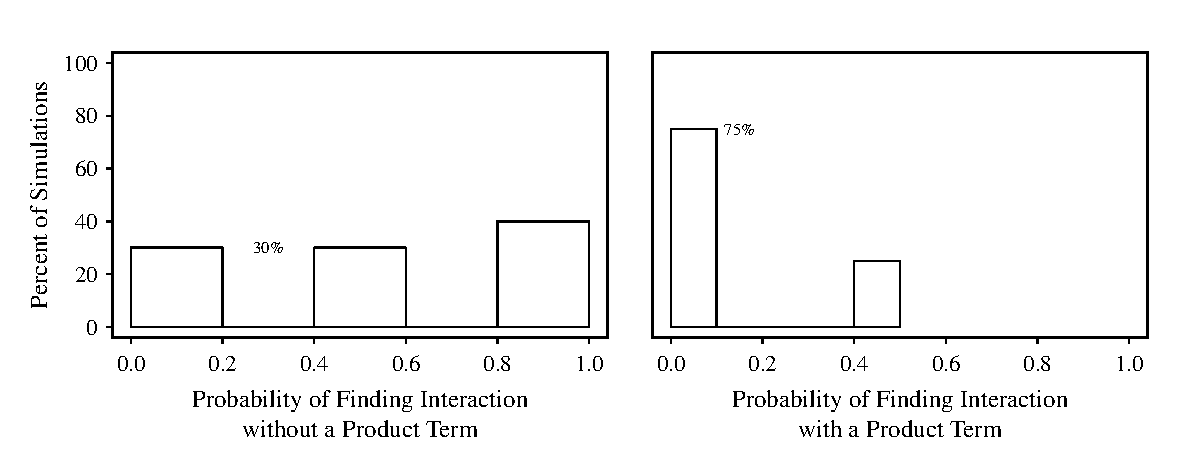
\includegraphics[scale = .7]{fig/fig-hist.pdf}
\end{center}\caption{The histogram on the left shows that logistic regression models without a product term tend to find interaction when none exists. The histogram on the right shows researchers can eliminate most of this bias by simply including a product term.}\label{fig:hist}
\end{figure}

Figure \ref{fig:scatter} directly compares the two approaches. Notice that every point falls below the diagonal line, except when both approaches fall below 0.1 (i.e., both perform well). This means that in every situation in which excluding a product term led to substantial bias, the model with a product term reduced this bias. In no case did the model without a product term perform substantially better than the model with a product term. Regardless of the absolute performance of each, the model with a product term performs at least as well as the model without a product term in all the analysis generated in my simulation, except when both perform well. In cases in which the model with a product term performs somewhat poorly (e.g., the probability of finding interaction is about 0.3, for example), the model without a product term performs terribly (e.g., the probability of finding interaction is nearly 1.00).
 
\begin{figure}[H]
\begin{center}
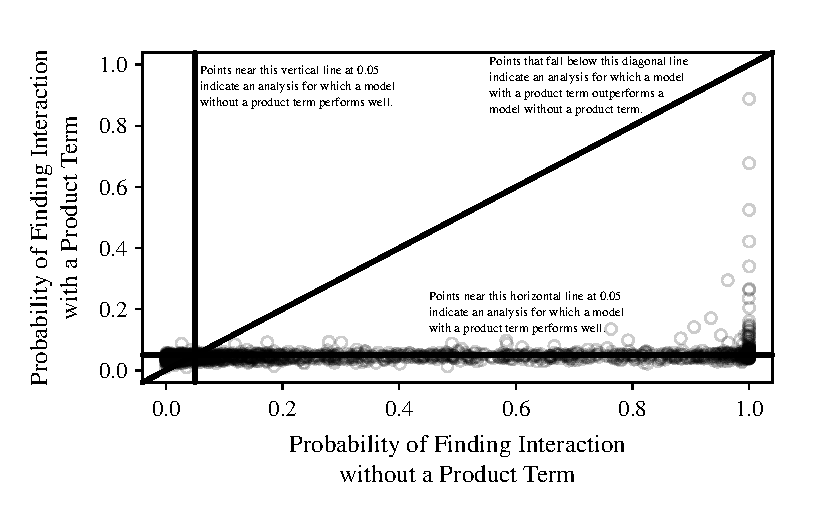
\includegraphics[scale = .9]{fig/fig-scatter2.pdf}
\end{center}\caption{This figure shows the probability of concluding interaction when none exists from logistic regression models with and without a product term for many different analyses. Notice that many points fall away from the vertical line at 0.05 indicating poor performance of models without a product term. Also notice that most points fall near the horizontal line at 0.05, indicating that models with a product term tend to perform well. Finally, notice that  all points fall below the diagonal line, indicating that models without a product term are more likely to mislead researchers in every simulated analysis.}\label{fig:scatter}
\end{figure}

\section*{Recommendations for Applied Researchers}

I suggest that applied researchers take several steps to ensure their claims of interaction are empirically meaningful.
\singlespace\vspace{-3mm}
\begin{enumerate}
\item Clearly explicate your interactive theory \citep{ClarkGilliganGolder2006, BerryGolderMilton2012} and carefully consider which relationships are consistent and inconsistent with the theory. Only use empirical models that can represent both relationships.
\item As \cite{BerryDeMerittEsarey2010} suggest, specify whether the relevant outcome variable is the latent variable $Y^*$ or the expected value $\text{Pr}(Y)$. If you use the concept $Y^*$, then test for interaction by testing the statistical significance of the product term. If you rely on $\text{Pr}(Y)$, then test for interaction by simulating confidence intervals around a carefully chosen second-difference or second-derivative. See \cite{BerryDeMerittEsarey2010} for the details of calculating a second-derivative or second-difference and \cite{KingTomzWhittenburg2000} for the details of the simulation procedure. Note that \cite{HanmerKalkan2013} offer an alternative approach in which researchers average the quantity of interest across the observed data rather than choosing a specific comparison of interest.
\item Regardless of whether the theoretically relevant outcome is $Y^*$ or $\text{Pr}(Y)$, and even if you theorize interaction on the basis of compression alone, you  must include product terms in order to draw compelling substantive conclusions about interaction from logistic regression models. Otherwise, you are simply pulling assumptions through data and treating them as conclusions.
\item As \cite{Nagler1991} and \cite{Frant1991} note, if you do not include a product term, then avoid making claims about interaction. The interaction is assumed and you should understand and clearly identify it as such.\footnote{Note that while researchers might suspect interaction between two variables (perhaps these are control variable), it is not necessary to include the product term as long as no empirical claim is made about the interaction of these variables. For example, it is not necessary for future studies of conflict to include the product of democracy and distance in their logistic regression models unless the researchers are specifically interested making compelling empirical arguments that the two interact in influencing the probability of conflict.}
\end{enumerate}
\doublespace

\section*{Democracy, Distance, and the Probability of Conflict}

To illustrate how to conduct a compelling test for interaction due to compression, I replicate analyses by \cite{OnealRusset2001}.\footnote{While \cite{OnealRusset2001} estimate several different model using generalized estimating equations, I estimate only their simplest logistic regression model (p. 314, Table A3.1) using maximum likelihood and the usual standard errors. Using their more complex approach does not substantively alter the results, though it does increase the standard errors slightly.}  \cite{BerryDeMerittEsarey2010} explain that the probability of war between two democracies is nearly zero, but much higher if one or both countries is non-democratic. Thus, on the basis of compression alone, \cite{BerryDeMerittEsarey2010} argue that one can meaningfully hypothesize that  explanatory variables should have smaller effects on the probability of conflict when both countries are democratic, simply because this probability is so close to zero. Using the example of geographic distance, the authors note that we should expect distance to have a much smaller effect on the probability of conflict when both countries are democracies than when at least one country is not democratic. Importantly, we have no reason to expect that democracy and distance interact in influencing the latent outcome (e.g., the utility of conflict). Thus, we have no reason to theorize about the sign of the product term. Further, the only reason to include a product term is to allow the model to represent a situation in which we are wrong (i.e., there is no interaction between democracy and distance in influencing the probability of conflict). 

This leads to three hypotheses about the effects of distance and democracy on the probability of conflict. First, as has been commonly suggested \citep[e.g.,][]{Ray1998, TomzWeeks2013}, democracies are much less likely to fight each other.

\begin{quote}
\textsc{Democracy Hypothesis}: Regardless of the distance between the two countries in a dyad, as the joint level of democracy in the dyad increases, the probability of conflict in that dyad decreases.
\end{quote}

Second, other literature in international relations points out that states that are located geographically further from one another are less likely to engage in conflict \citep[e.g.,][]{Diehl1991, Bremer1992}. 

\begin{quote}
\textsc{Distance Hypothesis}: Regardless of the level of democracy in the dyad, as the distance between the countries in the dyad increases, the probability of conflict in that dyad decreases.
\end{quote}

As \cite{BerryDeMerittEsarey2010} point out, these two hypotheses imply a third hypothesis. Because democratic dyads are much less likely to engage in conflict, we should expect the negative effect of distance to be much smaller in these dyads simply due to compression.

\begin{quote}
\textsc{Interaction Hypothesis}: The negative effect of distance on the probability of conflict is larger (more negative) in non-democratic dyads than in democratic dyads.
\end{quote}

\subsection*{Results}

 To test these three hypotheses, I use data from \cite{OnealRusset2001}. Their logistic regression model of  conflict (militarized interstate disputes) includes variables for democracy (smaller of the two Policy IV scores in each dyad), distance (the number of miles between the capitals), and several control variables. I estimated one model using Oneal and Russet's exact specification (with no product terms) and another model that includes the product of democracy and distance.\footnote{Oneal and Russet use generalized estimating equations (GEE) to estimate their models, but I rely on the simpler approach of maximum likelihood. The two methods produce substantively similar results, but the standard errors from the GEE approach are slightly larger. } See the Appendix for the details and the coefficient estimates. {The estimates from models with and without a product term are presented in the Appendix. } Since each of the hypotheses are stated in terms of the probability of conflict, I compute and plot estimates and 90\% confidence intervals for predicted probabilities, first-differences, and second-differences using CLARIFY-like simulation \citep{KingTomzWhittenburg2000}

Figure \ref{fig:pr-distance} provides a nice overview of the intuition and the evidence for the hypotheses by plotting the estimated probably of conflict  in both democracies and non-democracies from each empirical model.\footnote{Notice that the estimated relationships are similar across both modeling strategies. However, I have shown above that the model with no product term forces an interactive relationship into the results if both variables have an effect and the relevant probabilities are above or below one-half.} Notice that the results are consistent with all three hypotheses. First, increasing the distance between the states in a dyad reduces the probability of conflict in that dyad in both democratic (smallest Polity IV score is 10) and non-democratic (smallest Polity IV score is -10) dyads. Second, notice that the probability of conflict is lower in more democratic dyads, regardless of the distance between the states in the dyad. Finally, notice that the pacifying effect of distance is much smaller (i.e., less negative) in democratic dyads. 

        \begin{figure}[H]
        \begin{center}
        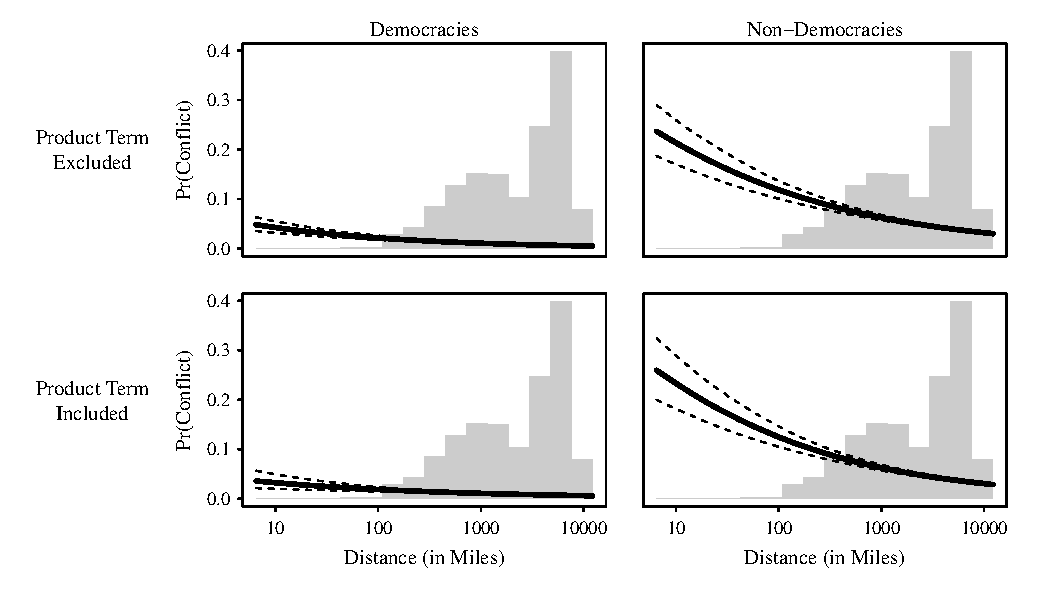
\includegraphics[scale = .8]{fig/fig-pr-distance.pdf}
        \end{center}\caption{This figure compares the estimated probability of conflict in democracies (Polity IV score of 10) and non-democracies (Polity IV score of -10) from models with and without a product term. Notice that, as expected, there is a much smaller change in the probability of conflict in democracies. However, the model with no product term forces this pattern of compression into the estimates. The model including a product term allows the model to represent non-interactive relationships as well. Because of this, the estimates from the model with a product term are more compelling.}\label{fig:pr-distance}
        \end{figure}

While the pattern of the predicted probabilities is consistent with the three hypotheses, I now compute and plot the quantities of direct substantive interest and the confidence intervals. First, Figure \ref{fig:pr-distance} plots the effect of moving from a non-democratic dyad (lower Polity IV score is -10) to a democratic dyad (lower Polity IV score is 10) on the probability of conflict as distance varies. The Democracy Hypothesis suggests that this effect should be negative regardless of the distance between the states. Figure \ref{fig:pr-distance} shows that the expected negative effect holds for across all distances and the confidence interval never overlaps zero. This pattern holds across the model with and without a product term.

        \begin{figure}[H]
        \begin{center}
        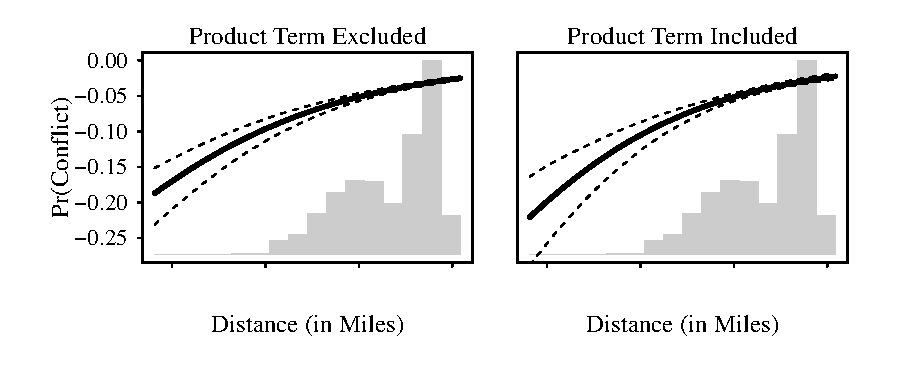
\includegraphics[scale = .8]{fig/fig-fd-distance.pdf}
        \end{center}\caption{This figure shows how the negative effect of distance on the probability of conflict shrinks toward zero as dyads become more democratic. This expected pattern is consistent with compression, but the model without a product term forces this pattern into the results while the model with a product term allows other types of relationships to emerge.}\label{fig:fd-distance}
        \end{figure}

Next, Figure \ref{fig:fd-democracy} plots the effect of moving from a ``nearby dyad'' (about 850 miles apart, which is the 25th percentile in the data set) to a ``distant dyad'' (about 8,600 miles apart, which is the 75th percentile) as the democracy of the dyad varies. The Distance Hypothesis predicts that this effect should be negative regardless of the level of democracy in the dyad. Figure \ref{fig:fd-democracy} shows that the effect is indeed negative across the range of observed levels of democracy and the confidence interval never overlaps zero. Again, this pattern holds across the models with and without a product term.
        
                \begin{figure}[H]
        \begin{center}
        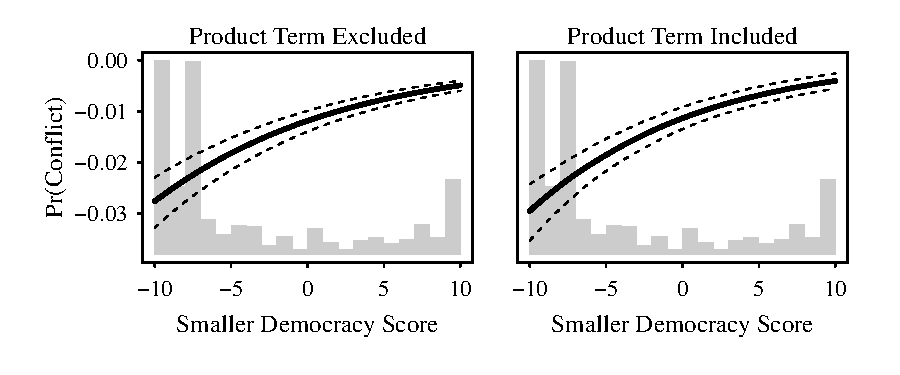
\includegraphics[scale = .8]{fig/fig-fd-democracy.pdf}
        \end{center}\caption{This figure shows how the negative effect of distance on the probability of conflict shrinks toward zero as dyads become more democratic. This expected pattern is consistent with compression, but the model without a product term forces this pattern into the results while the model with a product term allows other types of relationships to emerge.}\label{fig:fd-democracy}
        \end{figure}

Finally, and most importantly for my purposes, Figure \ref{fig:sd-distance} shows the estimated second-differences--the difference in the effects of distance among democratic and non-democratic states. The negative estimates suggest that distance has a smaller effect among democratic states, which supports the Interaction Hypothesis. Notice that, as before, the results are substantively similar across the model with and without a product term. Overall, then it seems that both models provide strong support for all three hypotheses. 

        \begin{figure}[h]
        \begin{center}
        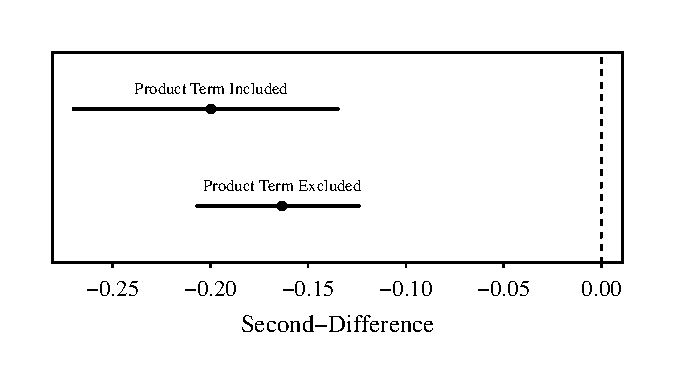
\includegraphics[scale = .8]{fig/fig-sd-distance.pdf}
        \end{center}\caption{This figure shows the estimated second-differences from both the models with and without a product term. While the estimates are similar, the results from the model with a product term are more compelling, because excluding a product term strongly biases the second-differences away from zero (see the left panel of Figure \ref{fig:plotted-cis}), while including removes most of this bias (see the right panel of Figure \ref{fig:plotted-cis}). }\label{fig:sd-distance}
        \end{figure}

\subsection*{Is Parsimony Preferable?}

When models with and without a product term provide similar (or nearly identical) conclusions, applied researchers might be tempted to discard the model with a product term for three reasons.
\singlespace\vspace{-3mm}
\begin{enumerate}
\item The logistic regression model with no product term captures the relationship (democracy and distance have negative effects and interact due to compression) suggested by the strong theory. \cite{BerryDeMerittEsarey2010} recommend excluding the product term in this situation.\footnote{\cite{BerryDeMerittEsarey2010} write: ``[A] researcher may have no reason to believe that the effects of independent variables on the latent variable $Y^*$ are interactive and may base his hypothesis that independent variables interact in influencing $\text{Pr}(Y)$ strictly on an expectation of compression. In this case, there is no need to include a product term in the model.''}
\item The AIC suggests the two models fit equally well (AIC = 13,520 for both models) and the BIC points toward the simpler with no product term (BIC = 13,580 for the model without the product term and BIC = 13,589 for the model with the product term). 
\item The product term is not statistically significant ($p = 0.23$). 
\end{enumerate}
\doublespace

Researchers might be tempted to drop the product term for \textit{any} of these three reasons. In spite of these temptations, \textit{parsimony is not preferable}. Researchers must include the product term $XZ$ when making arguments about $X$ and $Z$ interacting in influencing $\text{Pr}(Y)$. While the models might suggest similar conclusions, they do not offer similar \textit{evidence} for those conclusions. A model without a product term does not offer compelling evidence for interaction because it suggests interaction \textit{in spite} of the data, while a model with a product term suggests interaction \textit{because of} the data.

In the applied example, it is important to include the product term because it ``uncouples'' the Interaction Hypothesis from the Distance and Democracy Hypotheses. If I do not include a product term in the model, then the large negative effect of democracy and distance guarantee that the two interact in influencing $\text{Pr}(Y)$ (see the left panel of Figure \ref{fig:plotted-cis} and Equation \ref{eqn:dnoprod}). With no product term in the model, the Distance and Democracy Hypotheses \textit{imply} the Interaction Hypothesis and nothing is learned from examining the second-difference. By including the product term, however, I am able to uncouple the Democracy and Distance Hypotheses from the Interaction Hypotheses (see the right panel of Figure \ref{fig:plotted-cis} and Equation \ref{eqn:dprod}). When the model includes a product term, the Distance and Democracy Hypotheses no longer imply the Interaction Hypothesis and something is learned from examining the second-difference. While the two estimates of the second-difference presented in Figure \ref{fig:sd-distance} are similar, they represent different amounts of evidence for the Interaction Hypothesis. The estimate from the model with no product term is assumed by the structure of the empirical model. The estimate from the model with a product term, on the other hand, represents a meaningful relationship based on the data. 
\section*{Conclusion}

When researchers are interested in how explanatory variables interact in influencing the probability of an event, my study shows that (1) models \textit{without} a product term point toward interaction very often when none exists, (2) models \textit{with} a product term exhibit much less bias toward interaction, and (3) models \textit{with} a product term almost always reduce and usually eliminate the bias found in models \textit{without }a product term.  Although logistic regression models require ``compression''  to keep the probability of an event bounded between zero and one, researchers can limit the impact of this requirement on tests for interaction by simply including a product term, which allows the models to represent a  broad range of non-interactive relationships surprisingly well. Therefore, even when theorizing interaction due to compression alone, researchers should include a product term, making their theories more vulnerable to the data.\normalsize

\singlespace
\bibliographystyle{apsr_fs}
%\bibliography{/Users/rcrainey/Dropbox/Bibliography/bibliography.bib}
\bibliography{bibliography.bib}

\end{document}



